\documentclass{beamer}
\usetheme{CambridgeUS}
\usepackage{graphicx}
\usepackage{booktabs}
\usepackage{amsmath}
\usepackage{tikz}
\usepackage{listings}
\usepackage{xcolor}
\lstset{breaklines=true, basicstyle=\ttfamily\scriptsize}
\definecolor{nebulablue}{RGB}{25,118,210}
\definecolor{nebulagray}{RGB}{97,97,97}

\title[Nebula GPU Interconnect]{Nebula GPU Interconnect System:\\Technical Architecture and Implementation}
\author{Pranav Chandra, Pramit Pal, Meghadri Ghosh\\Team Bob}
\date{September 2025}

\AtBeginSection[]{
  \begin{frame}{Outline}
    \tableofcontents[currentsection]
  \end{frame}
}

\begin{document}

%-------------------------------------------------
\begin{frame}
  \titlepage
  \note{
    This presentation introduces the \textbf{Nebula GPU Interconnect System}, a scalable, cache-coherent NoC for multi-GPU communication. The work covers \textbf{mesh topology}, \textbf{protocol support}, \textbf{router microarchitecture}, and \textbf{verification}. Emphasize the \textbf{technical depth} and \textbf{design decisions} throughout.
  }
\end{frame}

% Table of Contents
\begin{frame}{Outline}
  \tableofcontents
\end{frame}

%-------------------------------------------------
\section{Project Overview}

\begin{frame}{Project Overview}
  \begin{itemize}
	\item \textbf{Output: }A scalable NOC design for multi-GPU system
	\item \textbf{Topology:} 2D mesh, 2x2 to 8x8 grid (up to 64 GPUs)
    \item \textbf{Protocols:} ARM AMBA AXI4 (non-coherent), CHI (coherent)
    \item \textbf{Languages Used:} SystemVerilog (RTL), Python (Analysis)
    \item \textbf{Key Features:}
      \begin{itemize}
        \item Five-stage router pipeline 
        \item Adaptive and deterministic routing
		\item Virtual channels for deadlock avoidance
		\item Credit based flow and arbitration
      \end{itemize}
  \end{itemize}
\end{frame}

%-------------------------------------------------
\section{The Packet}

\subsection{Packet Structure}
\begin{frame}{The Packet}
	\begin{columns}[T]
		\begin{column}{0.65\textwidth}
			\begin{itemize}
				\item Packets are sent as FLITs. Each packet consists of:
				\begin{itemize}
					\item \textbf{Header:} 48 bits
					\item \textbf{Payload:} 512 bits, data being transferred
					\item \textbf{Tail:} 32 bits, error checking and end of packet marker
				\end{itemize}
			\item Packets may be sent as single or multi-flit.
			\item Packets are usable in up to 16x16 meshes.
			\item QoS allows for packet prioritization.
			\end{itemize}
		\end{column}
		\begin{column}{0.3\textwidth}
			\begin{figure}
				\centering
				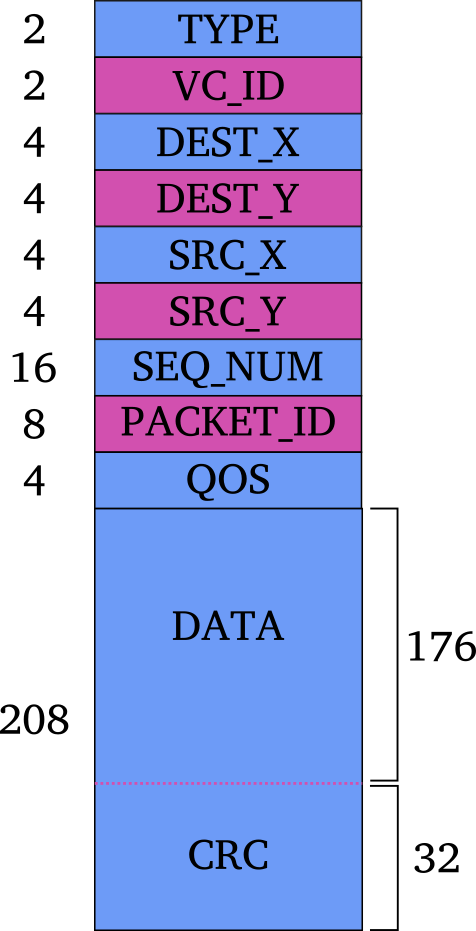
\includegraphics[width=0.8\linewidth]{images/packet-struct.png}
				\caption{Packet Structure}
			\end{figure}
		\end{column}
	\end{columns}
\end{frame}


\subsection{Packet Assembly and Disassembly}
\begin{frame}{Packet Assembly and Disassembly}
	\begin{itemize}
		\item Handled by \lstinline{nebula_packet_assembler.sv} and \lstinline{nebula_packet_disassembler.sv}.
\item Converts coordinates and metadata into predefined packets.
		\item Payload segmentation splits large payloads across multiple flits to optimize transmission.
		\item Ensures proper packet formation for both AXI4 and CHI protocols.
	\end{itemize}
\end{frame}

%-------------------------------------------------
\section{Router Microarchitecture}
\subsection{Router Overview}
\begin{frame}{Router Microarchitecture}
	\begin{itemize}
		\item Routers use a 5-stage pipeline for processing packets:
		\begin{enumerate}
			\item Buffer Write (BW)
			\item Route Computation (RC)
			\item Virtual Channel Allocation (VA)
			\item Switch Allocation (SA)
			\item Switch Traversal (ST)
		\end{enumerate}
		\item Routers have 5 ports each.
		\item Each port has 4 virtual channels (VCs).
		\item Each VC has a buffer depth of 8 flits.
		\item Four stage FSM to determine control.
	\end{itemize}
\end{frame}

\subsection{Router Pipeline Stages}
\begin{frame}{Buffer Write (BW)}
	\begin{itemize}
		\item Incoming flits are written to the appropriate VC buffer.
		\item Flow control is managed using a credit-based system.
		\item Ensures that buffers do not overflow.
	\end{itemize}
\end{frame}

\begin{frame}{Route Computation (RC)}
	\begin{itemize}
		\item Determines the next hop for the packet based on destination address.
		\item Implements XY routing algorithm for deadlock-free routing.
		\item Considers network congestion and adaptively selects paths.
	\end{itemize}
\end{frame}

\begin{frame}{Virtual Channel Allocation (VA)}
	\begin{itemize}
		\item Allocates a virtual channel for the packet to use on the next hop.
		\item Uses a round-robin arbitration scheme to ensure fairness.
		\item Prevents head-of-line blocking by allowing multiple packets to share physical channels.
	\end{itemize}
\end{frame}

\begin{frame}{Switch Allocation (SA)}
	\begin{itemize}
		\item Allocates the switch fabric to the selected virtual channel.
		\item Uses a priority-based arbitration scheme to resolve conflicts.
		\item Ensures that high-priority packets are transmitted first.
	\end{itemize}
\end{frame}

\begin{frame}{Switch Traversal (ST)}
	\begin{itemize}
		\item The packet is transmitted through the switch to the next router or destination.
		\item Updates credit counters for flow control.
		\item Ensures that packets are sent in the correct order.
	\end{itemize}
\end{frame}

\subsection{Router Control FSM}
\begin{frame}{Virtual Channel FSM}
	\begin{itemize}
		\item Each virtual channel maintains independent state, enabling concurrent packet processing across flows.
		\item The FSM follows a four-state cycle:
		\begin{enumerate}
			\item \textbf{IDLE} $\rightarrow$ awaits packet arrival
			\item \textbf{ROUTING} $\rightarrow$ performs route computation
			\item \textbf{WAITING VC} $\rightarrow$ waits for VC allocation
			\item \textbf{ACTIVE} $\rightarrow$ transmits flits, returns to IDLE after TAIL/SINGLE
		\end{enumerate}
		\item Transitions are driven by pipeline events: head/single flit arrival, route computation results, VC allocation success, and tail/single flit detection.
		\item Coordination relies on \texttt{rc\_valid}, \texttt{va\_valid}, switch arbitration signals, and generates \texttt{vc\_read\_en} for FIFO timing.
	\end{itemize}
\end{frame}

\subsection{Routing Algorithms}
\begin{frame}{Routing Algorithms}
	\begin{enumerate}
		\item Deterministic XY Routing
		\item Adaptive Routing
	\end{enumerate}
	\begin{columns}[b]
		\begin{column}{0.5\textwidth}
			\begin{figure}
				\centering
				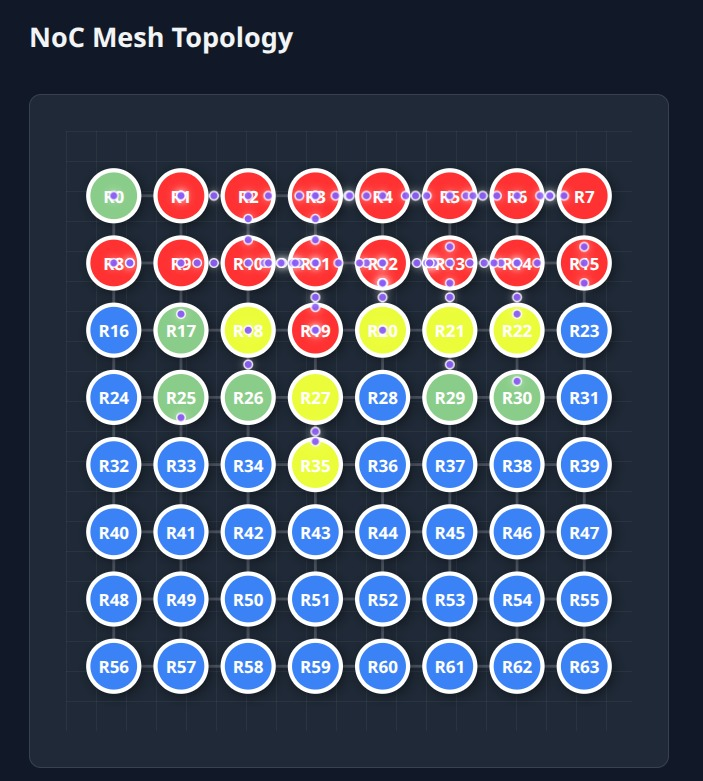
\includegraphics[width=0.6\linewidth]{images/xy-routing.jpg}
				\caption{XY Routing Example}
			\end{figure}
		\end{column}
		\begin{column}{0.5\textwidth}
			\begin{figure}
				\centering
				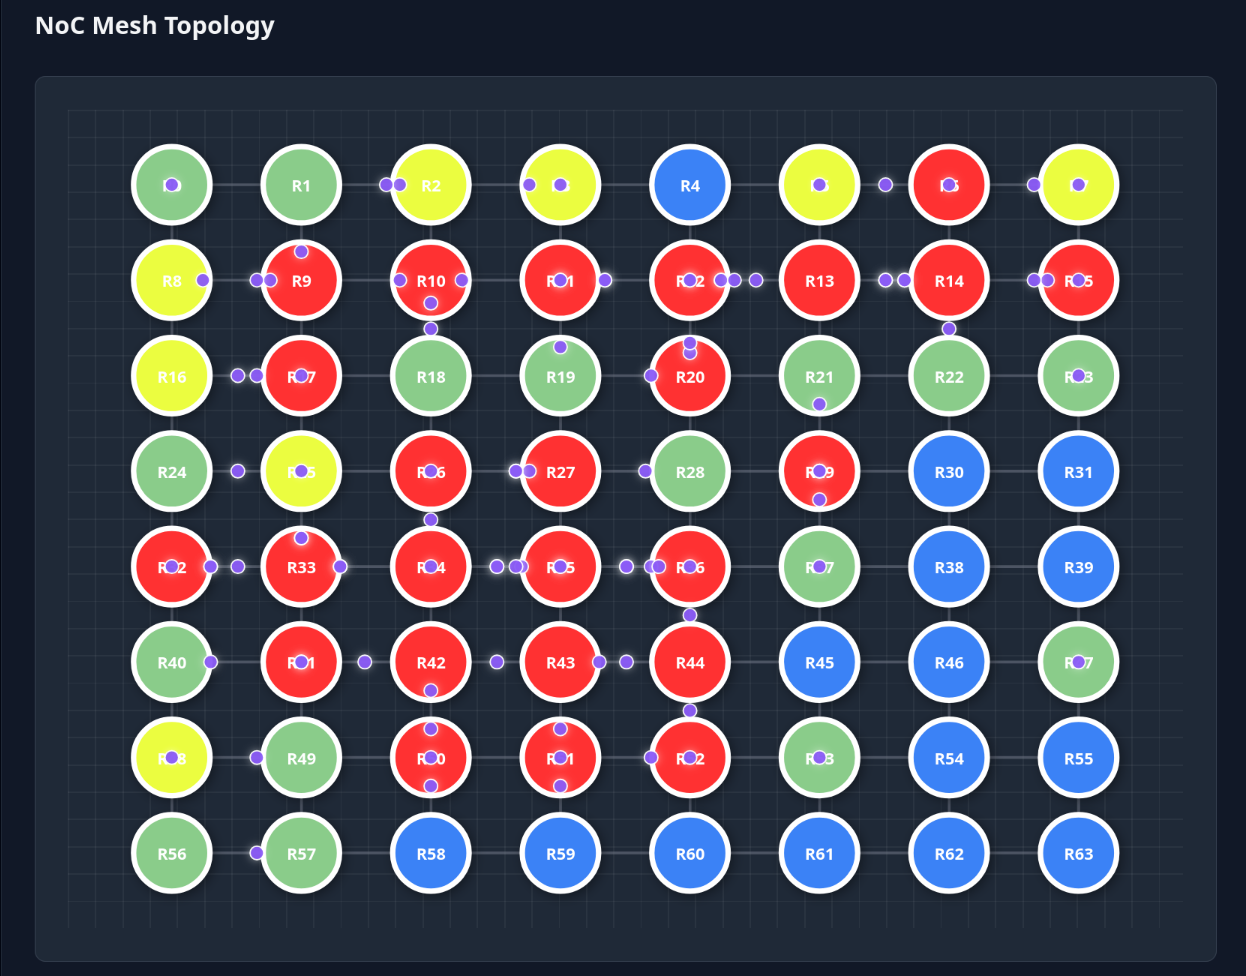
\includegraphics[width=0.8\linewidth]{images/adaptive-routing.png}
				\caption{Adaptive Routing Example}
			\end{figure}
		\end{column}
	\end{columns}
\end{frame}


\section{Credit Based Flow Control and Arbitration}
\subsection{Credit-Based Flow Control}
\begin{frame}{Credit-Based Flow Control}
  \begin{itemize}
    \item \textbf{Credit Controller (\texttt{nebula\_credit\_flow\_ctrl.sv}):}
      \begin{itemize}
        \item Per-VC credit counters, max 16
        \item Increment on flit acceptance, decrement on allocation
        \item Prevents buffer overflow, deadlock
        \item \texttt{credits\_available} signals for arbitration
      \end{itemize}
    \item \textbf{Flow Control Protocol:}
      \begin{itemize}
        \item Sender stalls if credits = 0
        \item Lossless operation guaranteed
      \end{itemize}
  \end{itemize}
\end{frame}

\subsection{Arbitration Mechanism}
\begin{frame}{Arbitration Mechanism}
\end{frame}

\section{Questions}
\begin{frame}{Questions}
  \begin{center}
	\Huge Questions?
  \end{center}
\end{frame}
\end{document}
